\chapter{Conclusion}
\label{chap:conclusion}

\minitoc

\graphicspath{{.}{chapitres/conclusion/}}

\section{Contribution Summary}
\label{sec:conclusion:contributions-summary}

\subsection{\dspot}
\label{subsec:conclusion:contributions-summary:dspot}

The major technical contribution of this thesis is an unit test amplification algorithm, implemented in a mature tool called \dspot.
\dspot aims at improving existing test methods with respect to a given test-criterion such as branch coverage.
It does this in 3 main steps.

1) It amplifies the input of the original test method by applying specific code transformation on the input part of the test method;

2) It removes existing assertions and generates new ones, based on observations done during execution on the state of the programs.
It uses commons getters in Java to do so.

3) It uses a test-criterion to select amplified test methods to keep.
For instance, one wants to improve the branch coverage of the test suite.
\dspot will keep only amplified test methods that cover branches that were not cover before.

\dspot has been developed in Java, for Java programs.
However, the whole technique remains applicable for all programming languages.

All the code of \dspot is available on \gh: \url{https://github.com/STAMP-project/dspot.git}.
I personally enliven its community by answering questions on the bug tracker, guiding new contributors and setting up methodologies, such as pull-request based development or integration continue, to keep \dspot as clean as possible.

Following this technical contribution, this thesis presented two large-scale evaluations of \dspot's effectiveness.

\subsection{Automatic Test Amplification For Mutation Score}
\label{subsec:conclusion:contributions-summary:test-ampl-ms}

For a first evaluation, I used \ms as test-criterion.
\dspot has automatically amplified test suites from open-source projects from \gh and improved the \ms.
%The \ms has been used as a proxy of test suites' ability to detect faults.

The generated amplified test methods of \dspot have been proposed to external developers of the projects from \gh through pull-requests.
This has been done in order to have the developers assessing the result of \dspot.
Over 19 opened pull-requests, 14 of them have been permanently added to the test suites of these projects.
It means that \dspot generated amplified test methods that are valuables for external developers.
%Everyday, amplified test methods are increasing the developers' confidence in the correctness of their software.

Also, I evaluated \dspot by amplifying 40 test classes of heavily tested projects from \gh, using also the \ms as test-criterion.
This evaluation shows that \dspot is able to generate amplified test methods that increase the \ms.

\subsection{Automatic Test Amplification For Behavioral Changes Detection}
\label{subsec:conclusion:contributions-summary:behavioral-change-detection}

In a second evaluation, I used \dspot in the context of continuous integration.
The goal was to generate amplified test methods that detect behavioral changes.

I took open-source projects from \gh and a selection of commits.
This evaluation showed that \dspot is able to generate amplified test methods that detect 25 behavioral change over 60, which is an achievement.
It also highlights the fact that \dspot can be easily implemented in the life cycle of software, like continuous integration.

This evaluation brings evidence that \dspot has to potential to be a concrete part of continuous integration by improving the process of program evolution with amplified test methods that are able to distinguish between versions of the same program.

\subsection{Transversal Contributions}
\label{subsec:conclusion:contributions-summary:transversal-contributions}

During this thesis, I developed a wide range of knowledge and skills that allowed me to participated to diversified and transversal contributions.

\subsubsection{Study of Program Correctness}
\label{subsubsec:conclusion:contributions-summary:transversal-contributions:correctness-attraction}

I devised a protocol, named \perturb, to study the programs' correctness under runtime perturbation.
Ten subjects have been studied using the PONE perturbations model, \ie adds 1 to integer expressions at runtime.
It results in 2,509,012 perturbed executions, which makes it one of the largest perturbation experiments ever made.
This large number come from the fact that the protocol explores exhaustively the perturbation space.
It allows to generalize the result over integer expressions.
From this experimentation, the presence of correctness attraction has been observed. 
Over all perturbed execution, 66\% of them do not break the correctness of the output, which is a important proportion. 
It means that software are quite reliable according to the PONE perturbations model.
For a large proportion, programs are able to recover from small perturbations and produce the correct output, assessed by perfect oracle.

\subsubsection{Study of Pseudo-tested Methods}
\label{subsubsec:conclusion:contributions-summary:transversal-contributions:pseudo-tested}

We replicated the study of \theoriginalauthors{} and confirmed that all Java projects contain \pseudotested{} methods, even the very well tested ones, ranging from 1\% to 46\% in our dataset.
From 3 projects, developers considered that 30\% methods were worthy of additional testing actions.
Pseudo-tested methods is an important issues since the coverage of the test suite ensures that the code is covered while it is not properly tested.
This is misleading and developers might think that the program is well tested while it is not.
Using test amplification to resolve this issue and test properly pseudo-tested methods is feasible.

\subsubsection{Study of Test Generation for Repair}
\label{subsubsec:conclusion:contributions-summary:transversal-contributions:test-for-repair}

To sum up, UnsatGuided can effectively alleviate the overfitting issue of regression introduction (16/19 cases), but has minimal positive impact on reducing the overfitting issue of incomplete fixing.
In this study, we used Evosuite, a state-of-the-art test generation tool.
An alternative would be to use a test amplification tool, such as \dspot in order to overcome the overfitting problems.

\section{Short-term Perspectives}
\label{sec:conclusion:short-prespectives}

In this section, I introduce short-term perspectives for \dspot.

1) Amplified test methods are based on existing ones.
The intuition would be that amplified test methods are easy to read as the seed test method.
However, since it is still an automatic process, the amplification can result in  difficult to read test methods.
A lacking key-feature is to make them prettier, and \autoref{subsec:conclusion:short-prespectives:prettifier} introduces a way to do it.

2) An obstacle of test amplification's tool adoption might be the way it must be used.
For example, \dspot is usable from command line with an executable jar or with a maven command.
Even if we put efforts to make this usage easier, developers might not want to type a command line, that can appear complex.
In \autoref{subsec:conclusion:short-prespectives:web-interface}, I introduce the idea of a web interface for test amplification tools.
This web interface would allow users to try test amplification tools, like \dspot, remotely using a graphic interface.
The ambitious of this is to spread test amplification approaches over open-source communities.
This would have 2 benefits:
1) Users would be welcomed with a friendly interface, and could discover test amplification step-by-step without modifying anything on their own computer.
2) It would collect data on the usage of test amplification and make a large experimentation thanks to users that, on their own, would use the amplification tool.

\subsection{Prettifying Amplified Test Methods}
\label{subsec:conclusion:short-prespectives:prettifier}

This section presents an algorithm that would make prettier amplified test methods.
Here prettier means that the amplified test method would have less noise, \ie would be easier to read for the developed.
In this context, I qualify as noise extra statements that are not required, redundant method calls or meaningless names from the generation process.
After applying this approach, the labels, \ie variables names and test method name, would be clear and carry the intent of the variable or of the test method and all extra statement would be removed.
This algorithm will take as input a set of amplified test methods, generated by a test amplification tool such as \dspot, and a test-criterion to output a set of prettier amplified test methods.
It will ensure that the prettified amplified test methods have the same quality than the input amplified test methods, with respect to the given test-criterion, \eg the \ms.

This algorithm would work in 3 main steps:

1) it would minimize the number of statement (\autoref{subsubsec:conclusion:short-prespectives:prettifier:miminize});

2) it would rename all the local variables with a name according to the context (\autoref{subsubsec:conclusion:short-prespectives:prettifier:rename-local});

3) it would rename the amplified test methods according to its body (\autoref{subsubsec:conclusion:short-prespectives:prettifier:rename-method}).

This workflow is summarize in \autoref{fig:dspot-prettifier-overview}.

Such algorithm could be evaluated by comparing how the algorithm would minimize an amplified test methods and a minimazation done manually by a developers.
Would the algorithm be faster than the human?
Would the algorithm obtain a better, a worse or as similar minimization than the human?

\begin{figure}
	\label{fig:dspot-prettifier-overview}
	\caption{Overview of DSpot-prettifier's approach.}
	\fbox{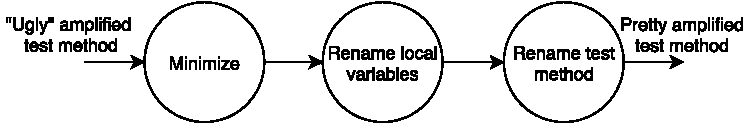
\includegraphics[width=.9\linewidth]{approach.pdf}}
\end{figure}

\subsubsection{Minimization}
\label{subsubsec:conclusion:short-prespectives:prettifier:miminize}
The minimization step would aim at reducing the size of the statement and the number statement to the minimal.
This would be done in 2 majors steps:

1) modifying the code using static analysis to avoid redundancy or useless local variable declaration;
The algorithm will replace multiple method calls, \eg to getters, that are the same by a local variable.
In the other way, it will replace local variables that are used only one time.

2) applying a search-based algorithm to remove the maximum number of statements, \emph{w.r.t.} to the specified test-criterion.
The intuition is as follow:
The algorithm would remove one statement;
it tries to compile the new test method;
if it fails, it means that this statement is needed to compile the test method and it must keep it;
otherwise, it measure the quality of the new test method according to the test criterion;
if it remains the same, it can remove the statement definitively, otherwise it cannot be removed;
It will repeat this process for all the statement inside the test method, starting by the end of the body.

\subsubsection{Rename Local Variables}
\label{subsubsec:conclusion:short-prespectives:prettifier:rename-local}

After that the algorithm would have minimize the statements, the next step would be to rename all the local variables.
The objectives would be to have variables with clear names, that give hints about the role and the intention of variables.

To do this, I could use Context2Name\footnote{\url{https://github.com/rbavishi/Context2Name}}\cite{DBLP:journals/corr/abs-1809-05193} which is a deep learning-based approach to infer natural variable names.
The idea behind Context2Name is to exploit the usage context, \ie the surrounding lexical tokens, of the variable to infer a proper name in natural languages.
For each local variables, the algorithm would use Context2Name to generate a new name for the local variable.


\subsubsection{Rename Amplified Test Method}
\label{subsubsec:conclusion:short-prespectives:prettifier:rename-method}

The final step would renaming the amplified test method.
This could be done in a similar way than renaming local variables \autoref{subsubsec:conclusion:short-prespectives:prettifier:rename-local} but at the method level.
The goal would be to have a clear name for the amplified test methods that give directly the intention of the test method.
In this way, developers would understand quicker what is the purpose of this test method
The major stake would be that developers are more likely to integrate amplified test methods into their test suite.

To do this, I could use Code2Vec\footnote{\url{https://github.com/tech-srl/code2vec}}\cite{DBLP:journals/corr/abs-1803-09473} which is a neural network for learning distributed representations of code.
However, since Code2Vec would use the whole body the test method, it would be mandatory that the algorithm renames the local variables before the amplified test methods.

\subsection{Collecting  Developers Feedback}
\label{subsec:conclusion:short-prespectives:web-interface}
The idea would be to provide to users a web interface, on which the user would have simply to put the URL of its \gh repository.
Then, we would retrieve the project and run \dspot on it.
This idea is largely inspired by CommitGuru\footnote{\url{http://commit.guru/}}\cite{Rosen:2015:FSE}.
CommitGuru is a tool that identifies and predicts risky software commits.
The user gives the URL of its git repository, \eg on github, and CommitGuru analyzes the project and its commits to highlights potential threats.

The goal of this web interface would be to allow new users discover test amplification tools.
The users could consult the result of the amplification from the web interface, or by receiving an email.
All the data could be accessed from the web interface in order to allow the reproduction of test amplifications.

A UI mockup of the web interface is shown in \autoref{fig:dspot-web}.
On this picture, one can see that the users would have only to put the url of its repository and its email, in order to receive the result for example.
At the bottom, on can see a list of projects that used recently the test amplification tool.

\begin{figure}
	\centering
	\caption{Screenshot of the web interface for \dspot.}
	\label{fig:dspot-web}
	\fbox{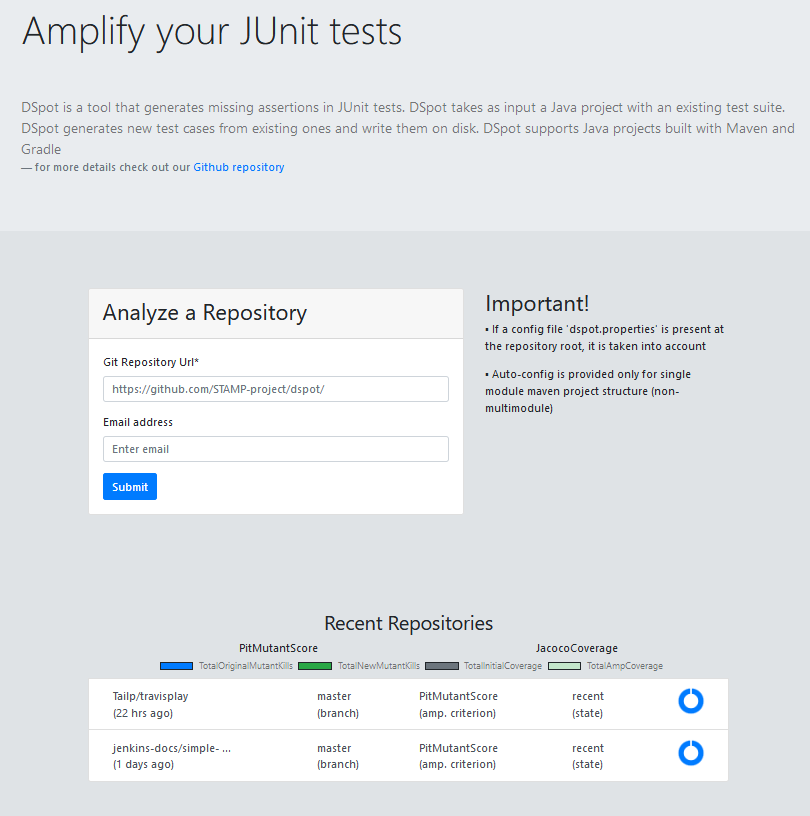
\includegraphics[width=0.9\textwidth]{dspot-web-1.png}}
\end{figure}

\section{Long-term Perspectives}
\label{sec:conclusion:long-prespectives}

In my vision, there are 2 long-term perspectives for \dspot:

1) sometimes, test-improvement resulting from a given test class should not be in the same class, \eg \autoref{subsubsec:test-improvement:experiment-results:rq1:mustache}.
This might be a limitation on the adoption of test amplification tools by industrials since they might be confused by the fact that the component tested is not any more related to the original test class.
\textbf{Would we able to find the best location for a given amplified test methods?}
This new location would take into account 2 aspect:
1) objects used in the test and the methods called on then, \ie the input part.
2) the values that are asserted, \ie the oracle part.

2) Inspired from Repairnator~\cite{urli:hal-01691496}, which is bot that automatically executes test-based repairs programs to fix CI build failures.
Repairnator crawls builds status on Travis, a continuous integration service on \gh.
Then, Repairnator launches automatic repair tools to failing builds and then, it is able to propose the patch throught a pull-request on the \gh repository.
\textbf{Would we able to automatically amplify test suite from the CI and provide an test method that a developer did not?}
In the same way, we could imagine a bot that uses test amplification tools.
For example, the bot would launch \dspot on passing build, a contrario than Repairnator is executed on failing build, to amplify the test suite.
The goal of this amplification would be even to make evolve the test suite using the \ms as test-criterion such as shown in \autoref{sec:test-improvement:mutation-score} or to detect a regression such as shown in \autoref{subsec:dci:background:behavioral-change-detection}.
